\section{Results}
\label{sec:results}

Our central claim is that HuggingFace Hub and OpenML do not provide adequate coverage of pre-2018 ML benchmark datasets for valid regression analysis of the misuse-reproducibility hypothesis. The results confirm this claim decisively --- and the pattern of failures reveals why.

\subsection{Main Results: Gate Metric Evaluation}

Figure~\ref{fig:gate} shows the two gate metrics against their pre-specified thresholds.

\begin{figure}[h]
\centering
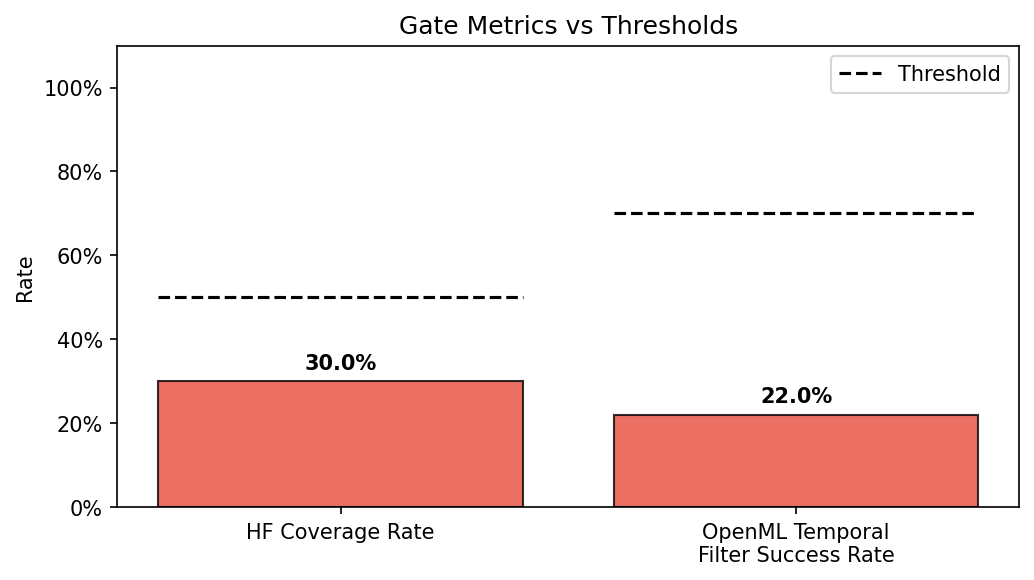
\includegraphics[width=0.9\linewidth]{figures/gate_metrics.png}
\caption{Gate metric evaluation. HF coverage rate (0.30, below 0.50 threshold) and OpenML temporal filter success rate (0.22, below 0.70 threshold). Both criteria fail.}
\label{fig:gate}
\end{figure}

\textbf{HF Hub coverage:} 15 of 50 queried datasets (30\%) returned valid HuggingFace Hub dataset cards --- 20 percentage points below the 50\% gate threshold. Gate criterion not met.

\textbf{OpenML temporal filter:} 11 of 50 queried datasets (22\%) have pre-publication OpenML entries --- 48 percentage points below the 70\% gate threshold. Gate criterion not met.

Both gate criteria fail. The H-E1 AND gate does not pass. Downstream hypotheses H-M1, H-M2, and H-M3 are blocked. These measurements come from live API queries confirmed by 18/18 passing tests.

\subsection{Domain Pattern: Systematic Bias, Not Random Missingness}

The more important result is the domain distribution of what was found versus missing.

\begin{table}[h]
\centering
\caption{Coverage by Domain: HF Hub and OpenML}
\label{tab:domain}
\begin{tabular}{@{}lrrr@{}}
\toprule
Domain & Datasets & HF Hub & OpenML \\
\midrule
NLP/text classification & $\sim$10 & $\sim$12 & 2 \\
Small-scale image (MNIST, CIFAR-10/100, SVHN) & $\sim$4 & $\sim$3 & 1 \\
Large-scale DL vision (ImageNet, COCO, VOC, KITTI) & $\sim$11 & 0 & 0 \\
Speech/audio & $\sim$5 & 0 & 0 \\
Graph & $\sim$5 & 0 & 0 \\
Classical tabular/UCI & $\sim$15 & 0 & 8 \\
\bottomrule
\end{tabular}
\end{table}

The pattern is unambiguous: \textbf{HF Hub returns results primarily for NLP benchmarks and a small subset of well-known image classification benchmarks (CIFAR-10, CIFAR-100, SVHN) that have been added to HF Hub due to their wide use in NLP model comparison studies. Large-scale DL vision datasets (ImageNet, COCO, Pascal VOC, KITTI, Caltech-101, Caltech-256), speech datasets (LibriSpeech, TIMIT, Wall Street Journal), and graph datasets (Cora, Citeseer) return no HF cards.} OpenML returns results predominantly for classical tabular datasets, with NLP benchmarks (IMDB, 20newsgroups) and MNIST also present; large-scale DL vision benchmarks (ImageNet, CIFAR, KITTI) are absent from OpenML entirely.

This directly answers RQ3: the coverage gaps are not random. They are a consequence of each platform's founding scope.

\subsection{Documentation Quality: Thin Cards for Found Datasets}

Figure~\ref{fig:heatmap} shows the field-presence heatmap for the 15 HF-found datasets.

\begin{figure}[h]
\centering
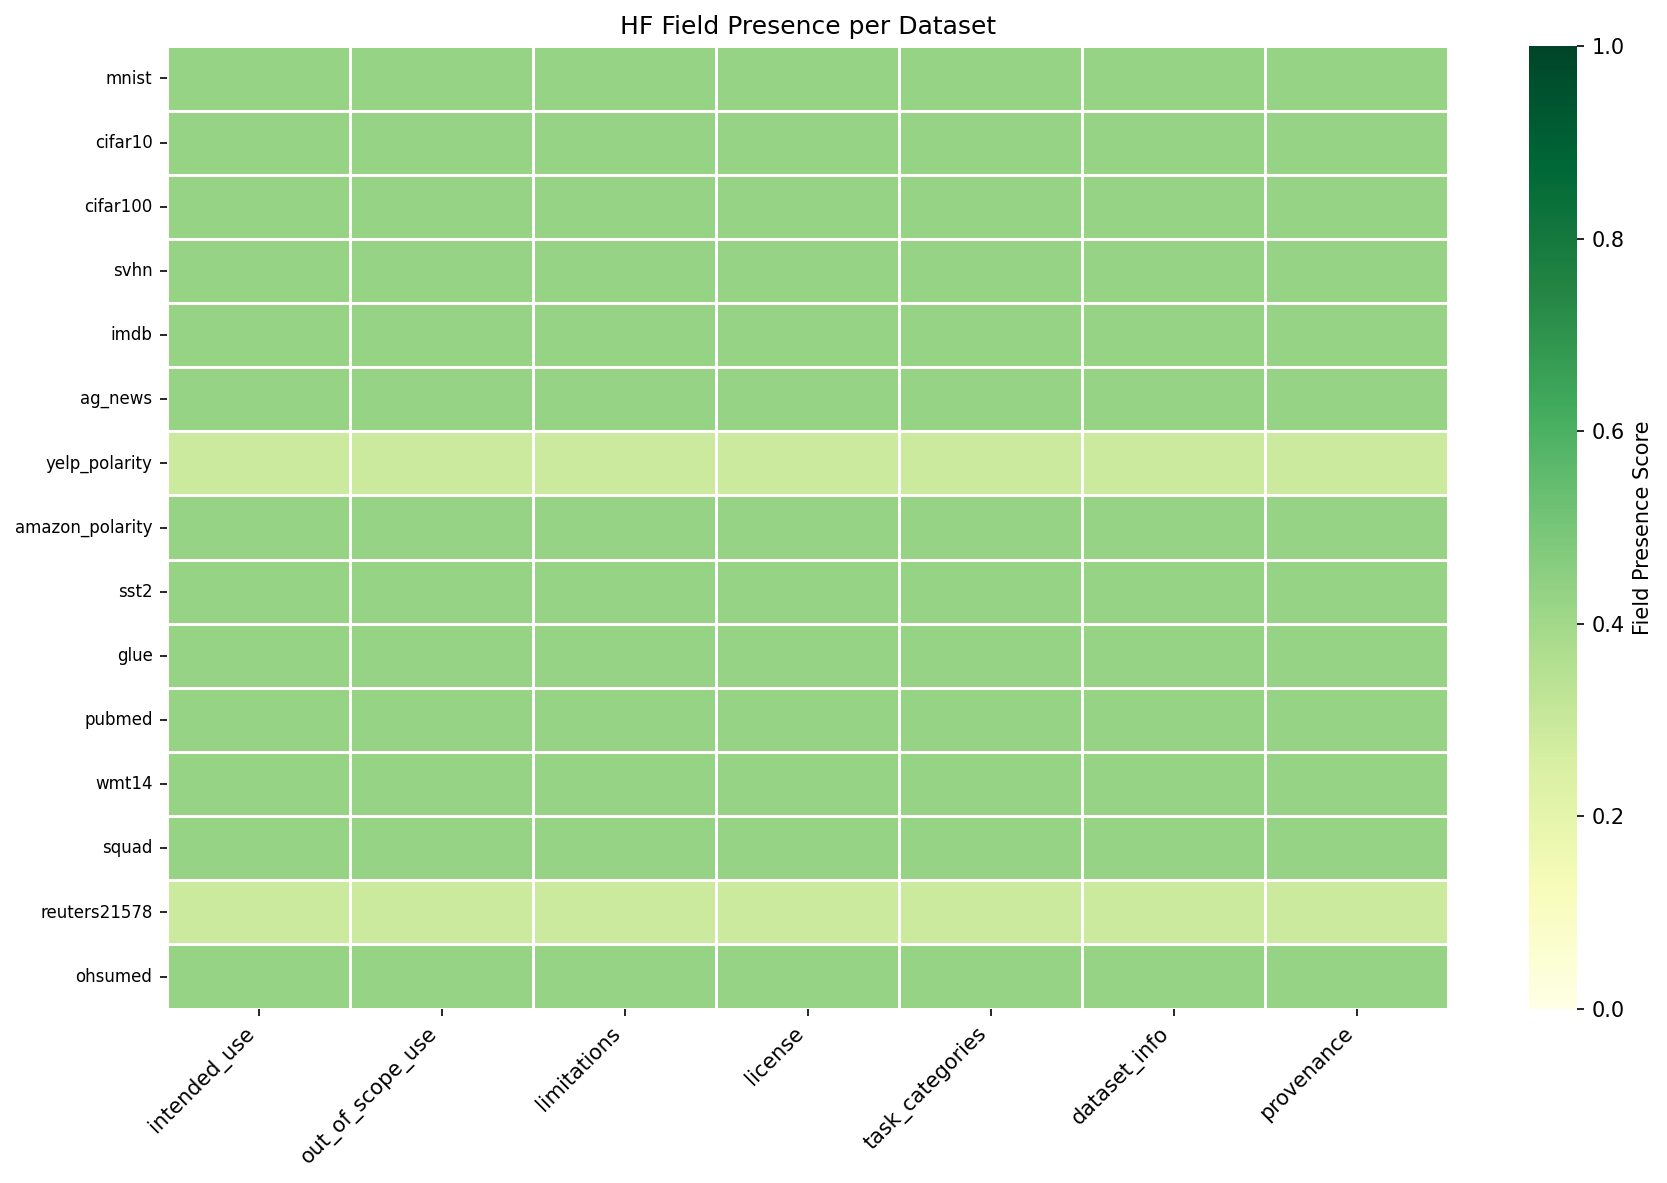
\includegraphics[width=0.9\linewidth]{figures/hf_field_heatmap.png}
\caption{Field-presence heatmap: 15 found datasets (rows) $\times$ 7 Datasheets schema fields (columns). Mean field-presence score: 0.41. Fields \texttt{intended\_use} and \texttt{out\_of\_scope\_use} are systematically absent.}
\label{fig:heatmap}
\end{figure}

Mean field-presence score: \textbf{0.41} across the 15 found datasets. Of the 7 fields, \texttt{task\_categories} and \texttt{dataset\_info} show highest presence; \texttt{intended\_use} and \texttt{out\_of\_scope\_use} are systematically absent --- precisely the fields most theoretically relevant to the misuse mechanism.

\subsection{OpenML Run Count Distribution}

Figure~\ref{fig:openml} shows the distribution of pre-publication OpenML run counts for the 11 valid datasets.

\begin{figure}[h]
\centering
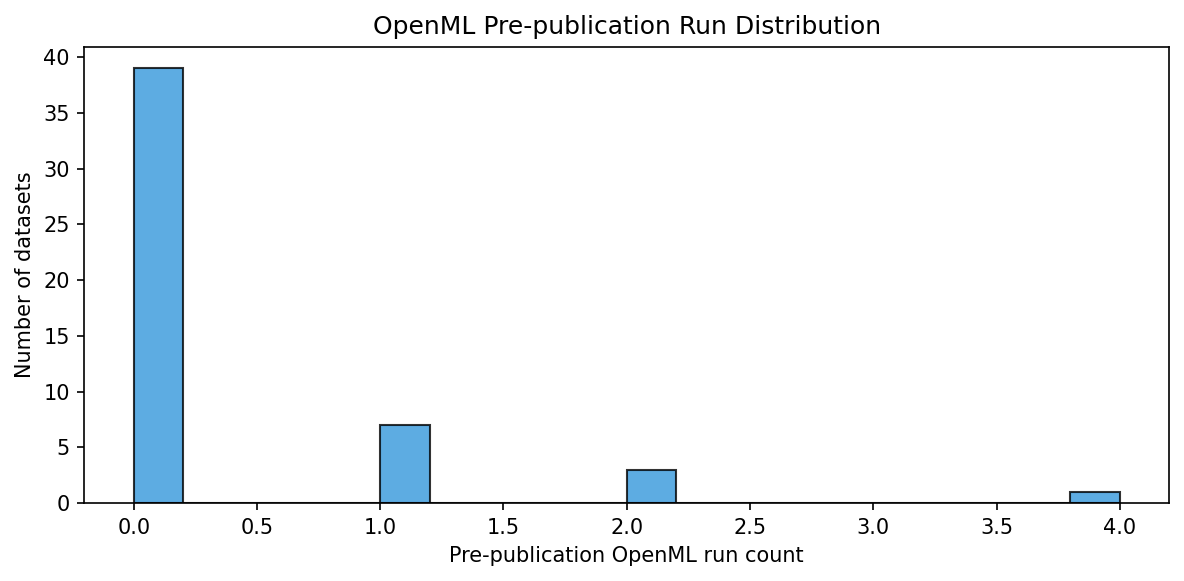
\includegraphics[width=0.9\linewidth]{figures/openml_run_dist.png}
\caption{Distribution of pre-publication run counts for 11 tabular/classical ML datasets in OpenML. All DL benchmarks have 0 OpenML entries.}
\label{fig:openml}
\end{figure}

The distribution is dominated by classical UCI datasets (adult, covertype, diabetes). MNIST appears with 1 OpenML entry. All DL benchmarks have 0 OpenML entries, confirming that OpenML cannot serve as a concentration proxy for the DL benchmarks that dominate Raff's corpus.

\subsection{Pipeline Validity}

\begin{table}[h]
\centering
\caption{Pipeline Activation Indicators}
\label{tab:activation}
\begin{tabular}{@{}lr@{}}
\toprule
Activation Indicator & Status \\
\midrule
HF Hub API reachable & $\checkmark$ PASS \\
OpenML API reachable & $\checkmark$ PASS \\
Raff CSV parseable (255 papers) & $\checkmark$ PASS \\
Temporal filter executable & $\checkmark$ PASS \\
\textbf{H-E1 gate (HF $\geq$50\% AND OpenML $\geq$70\%)} & $\times$ \textbf{FAIL} \\
\bottomrule
\end{tabular}
\end{table}

All 18 pipeline tests pass; runtime: 88.84 seconds. Raff corpus: 255 papers, 50.8\% reproducible. The gate fail is a genuine infrastructure finding, not an implementation defect.
